%!TEX encoding = UTF-8 Unicode

%!TEX root = ../compendium.tex

\Lab{\LabWeekFIVE}

\begin{Goals}
\item Kunna skapa och använda sekvenssamlingar.
\item Kunna använda sekvensalgoritmen SHUFFLE för blandning på plats av innehållet i en array.
\item Kunna registrera antalet förekomster av olika värden i en sekvens.
\end{Goals}

\begin{Preparations}
\item \DoExercise{\ExeWeekFIVE}{05}
\item Läs igenom hela labborationenen och säkerställ att du förstår hur SHUFFLE-algoritmen nedan fungerar.
\end{Preparations}

\subsection{Bakgrund}

Denna labb handlar om kortblandning. Att blanda kort så att varje möjlig permutation (ordning som korten ligger i) är lika sannolik är icke-trivialt; en osystematiskt blandning leder till en skev fördelning. 

Givet en bra slumpgenerator går det att blanda en kortlek genom att lägga alla kort i en hög och sedan ta ett slumpvist kort från högen och lägga det överst i leken, tills alla kort ligger i leken. Fisher-Yates-algoritmen\footnote{\href{https://en.wikipedia.org/wiki/Fisher\%E2\%80\%93Yates_shuffle}{https://en.wikipedia.org/wiki/Fisher\%E2\%80\%93Yates\_shuffle}} (även kallad Knuth-shuffle), fungerar på det sättet. Här benämner vi denna algoritm SHUFFLE. Den återfinns i pseudokod nedan:

\begin{algorithm}[H]
 \SetKwInOut{Input}{Indata}
 \Input{Array $xs$ som ska blandas}
 $len \leftarrow$ antalet element i $xs$ \\
 \For{$i \leftarrow (len - 1)$ \KwTo $0$}{
  $r \leftarrow$ slumptal mellan $0$ och $i$ \\
  $temp \leftarrow xs(i)$ \\
  $xs(i) \leftarrow xs(r)$ \\
  $xs(r) \leftarrow temp$ \\
 }
\end{algorithm}

Kortspelet poker handlar om att dra kort och få upp vissa kombinationer av kort, s.k. ''händer''\footnote{\href{https://sv.wikipedia.org/wiki/Pokerhand}{https://sv.wikipedia.org/wiki/Pokerhand}}. Dessa är ordnade från bättre till sämre; den spelare vinner som fått bäst hand.
Det är därför intressant att veta med vilken sannolikhet en viss hand dyker upp vid dragning från en blandad kortlek.

De vanliga pokerhänderna är, i fallande värde, färgstege (straight flush), fyrtal, kåk (full house), färg (flush), stege (straight), triss, tvåpar och par. Dessa finns illustrerade i labbhandledningen.
Ofta finns ytterligare en hand, s.k. ''royal flush'', men dess sannolikhet är för låg för att kunna simuleras fram på rimlig tid.

Under laborationen ska du börja med att göra klar den ofärdiga klassen \code{CardDeck} som visas nedan, och återfinns i laborationens workspace som du kan ladda ner från \url{http://cs.lth.se/pgk/ws} och importera i en IDE enligt instruktioner i appendix \ref{appendix:ide}. 

\scalainputlisting[numbers=left,basicstyle=\ttfamily\fontsize{10}{12}\selectfont]{../workspace/w05_shuffle/src/main/scala/cardSimulation/CardDeck.scala}

\noindent Labbinstruktionerna i avsnitt \ref{subsection:lab:shuffle:tasks} ger tips om hur du ska ersätta \code{???} i givna kodskellett med med dina lösningar. 

Efter att du testat så att din implementation av \code{CardDeck} fungerar, ska du använda \code{CardDeck} tillsammans med andra klasser som beskrivs nedan för att ta reda på sannolikheter för att olika pokerhänder uppkommer när man delar ut 5 kort ur en bra  blandad kortlek.

Till din hjälp har du ett antal färdiga kodfiler och en del ofärdig kod som du ska färdigställa. Alla klasserna ligger i ett paket med namnet \code{CardSimulation}. 

De givna kodfilerna är:\footnote{Du kan bläddra bland klasserna i paketet cardSimulation här: \\
\href{https://github.com/lunduniversity/introprog/tree/master/workspace/w05_shuffle/src/main/scala/cardSimulation}{\mbox{\fontsize{9}{11}\selectfont  https://github.com/lunduniversity/introprog/tree/master/workspace/w05\_shuffle/src/main/scala/cardSimulation}}}

\begin{itemize}
\item \code{CardDeck.scala} innehåller en klass som har en kortlek som kan blandas. Kompanjonsobjektet har en main-metod som skapar en kortlek, skriver ut, blandar och skriver ut.
\item \code{Card.scala} innehåller en \code{case class Card(suit: Int, value: Int)} som representerar ett kort och har en koncis \code{toString} med färg \Eng{suit} och valör.
\item \code{Hand.scala} innehåller en \code{case class Hand(cards: Vector[Card])} som representerar en pokerhand och har metoder för att avgöra vilken handen det är. I kompanjonsobjektet finns en fabriksmetod som kan skapa en hand genom att dra fem kort från en kortlek.
\item \code{PokerProbability.scala} har en main-metod som testar pokersannolikheter, samt ett par metoder som hjälper denna.
\item \code{TestingDeck.scala} är en nedskalad subklass till \code{CardDeck} som endast innehåller tre kort. Main-metoden i dess kompanjonsobjekt testar implementationen av \code{shuffle} och redovisar resultatet i ASCII-grafik.
\item \code{AsciiBarGraph.scala} innehåller enbart en metod som skapar ett stapeldiagram åt \code{TestingDeck}
\end{itemize}




\subsection{Obligatoriska uppgifter}\label{subsection:lab:shuffle:tasks}

\Task Implementera algoritmen SHUFFLE.

\Subtask Implementera metoden \code{shuffle} i klassen \code{CardDeck}. Följ algoritmen noga, och använd \code{cards.length} för att få fram längden på kortleken. 

\Subtask Kör \code{TestingDeck} för att testa att blandningen är jämnt fördelad. \code{TestingDeck} blandar en kortlek med tre kort och räknar hur ofta olika permutationer dyker upp. Du bör få en utskrift med sex ($3!$) ungefär lika långa staplar.

\Task Fyll i de ofärdiga delarna av klassen \code{CardDeck}.

\Subtask Skriv kod för att skapa en array innehållande en 52-korts standardlek. Använd konstanterna i \code{Card}. Tänk på att en \code{for}/\code{yield}-sats inte nödvändigtvis ger en \code{Array}, men att alla samlingar kan omvandlas till en sådan med \code{toArray}.

\Subtask Kör \code{CardDeck} och kontrollera så att du får kort av alla fyra färger, och både ess och kungar.

\Task Använd den färdiga \code{CardDeck}-klassen för att ta fram sannolikheterna för att  ''straight flush'', ''straight'' eller ''flush'' dyker upp.

\Subtask Implementera funktionen \code{test} i \code{PokerProbability}. Använd de färdiga funktionerna \code{Hand.drawFrom} och \code{testHand} för att dra och klassificera en hand från en kortlek. Lagra frekvenserna i en muterbar \code{Map} (\code{collection.mutable.Map} finns redan importerad).

\Subtask Kör \code{PokerProbability}, förslagsvis med 1000 000 iterationer. Du bör få ungefär dessa sannolikheter: 
\begin{figure}[H]\centering
\begin{tabular}{r|l}
\emph{hand} & $\emph{sannolikhet}$ \\ \hline
Straight flush & 0.00154\%  \\
Flush          & 0.197\%    \\
Straight       & 0.39\%     \\
High card      & 99.41\%
\end{tabular}
\end{figure}


\subsection{Frivilliga extrauppgifter}

\Task Implementera metoden \code{tally} i klassen \code{Hand} så att simuleringen även kan registrera kortkombinationerna fyrtal, kåk, triss, tvåpar och par. Kör sedan \code{PokerProbability} igen.


\Task Implementera ett interaktivt kortspel, t.ex. någon enkel pokervariant. Börja med något mycket enkelt och bygg vidare med sådant som du tycker verkar roligt. 



\subsection{Bilder med exempel på olika pokerhänder}

Figurerna \ref{lab:shuffle:first-picture} -- \ref{lab:shuffle:last-picture} visar bilder på olika korthänder i poker.

\begin{figure}[H]
 \begin{minipage}[c]{0.5\textwidth}
  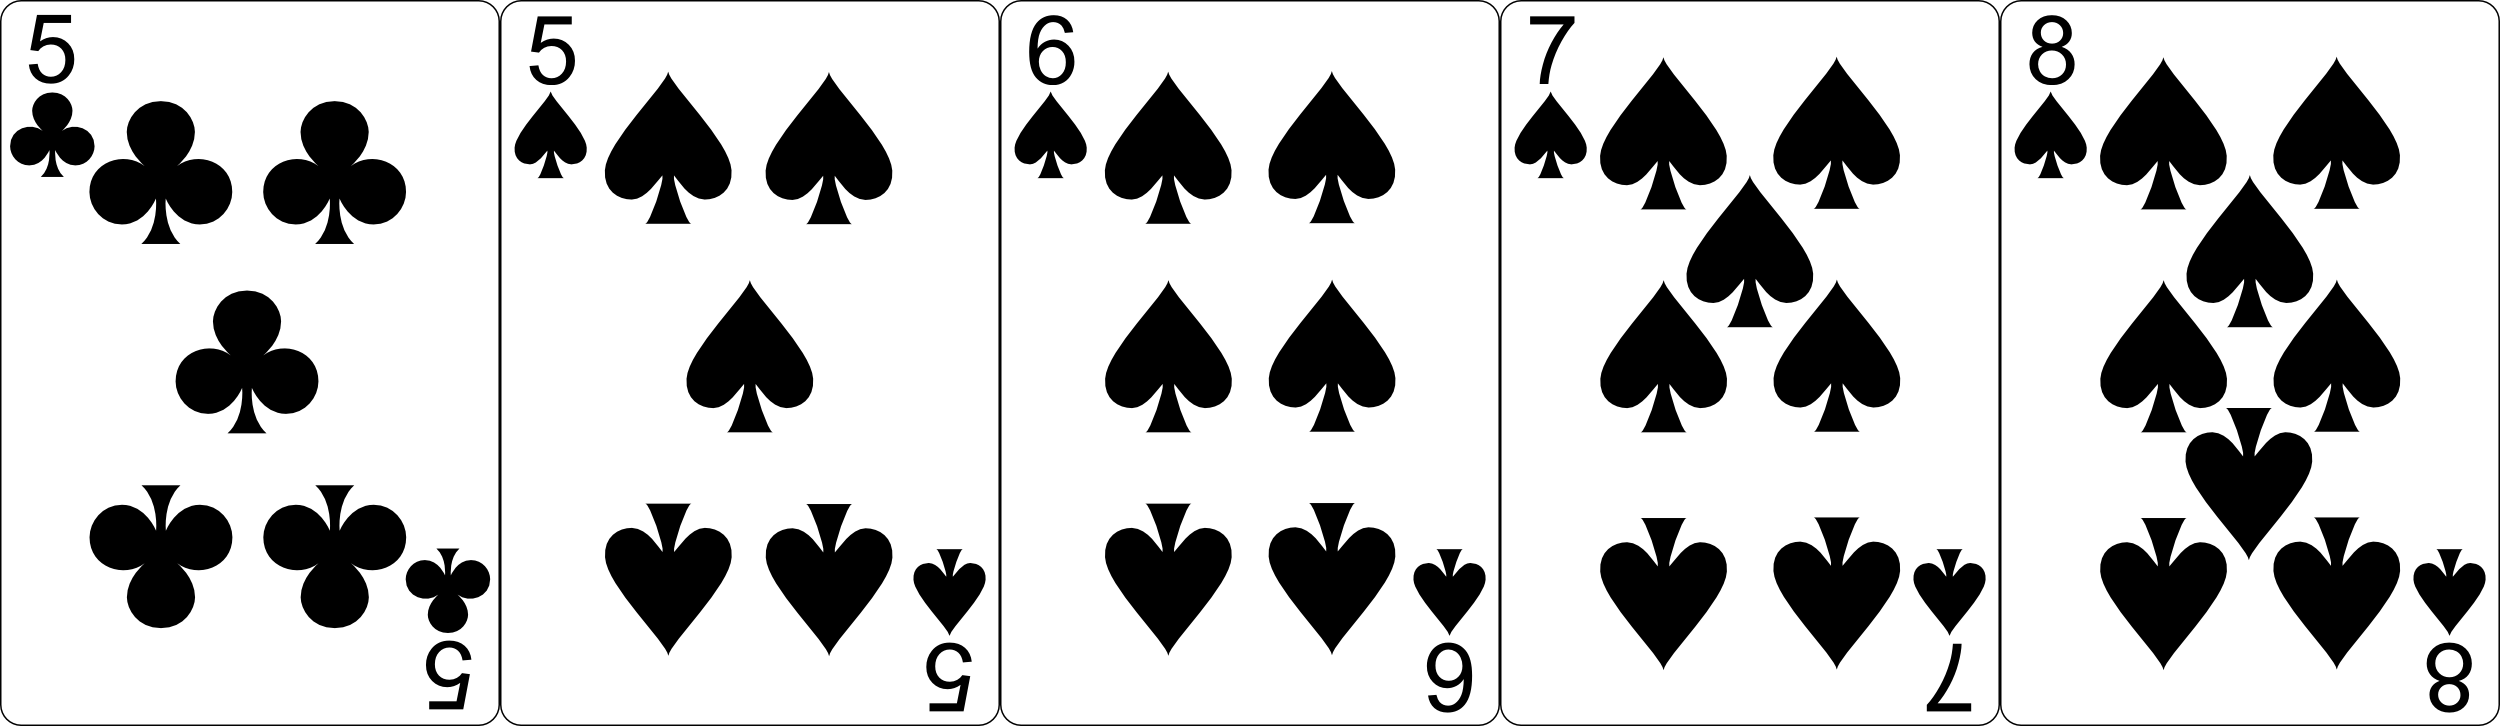
\includegraphics[width=\textwidth]{../img/w05-hands/pair.png}
 \end{minipage}
 \begin{minipage}[c]{0.3\textwidth}
  \caption{Par - två kort har samma valör}
   \label{lab:shuffle:first-picture}
 \end{minipage}
\end{figure}

\begin{figure}[H]
 \begin{minipage}[c]{0.5\textwidth}
  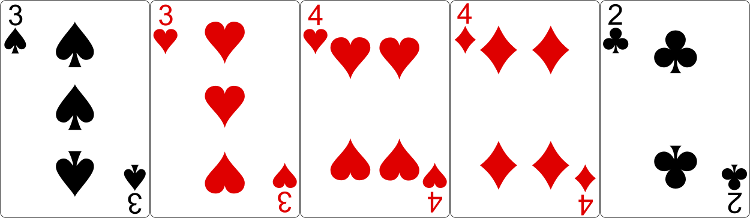
\includegraphics[width=\textwidth]{../img/w05-hands/twopair.png}
 \end{minipage}
 \begin{minipage}[c]{0.3\textwidth}
  \caption{Tvåpar - två olika par}
 \end{minipage}
\end{figure}

\begin{figure}[H]
 \begin{minipage}[c]{0.5\textwidth}
  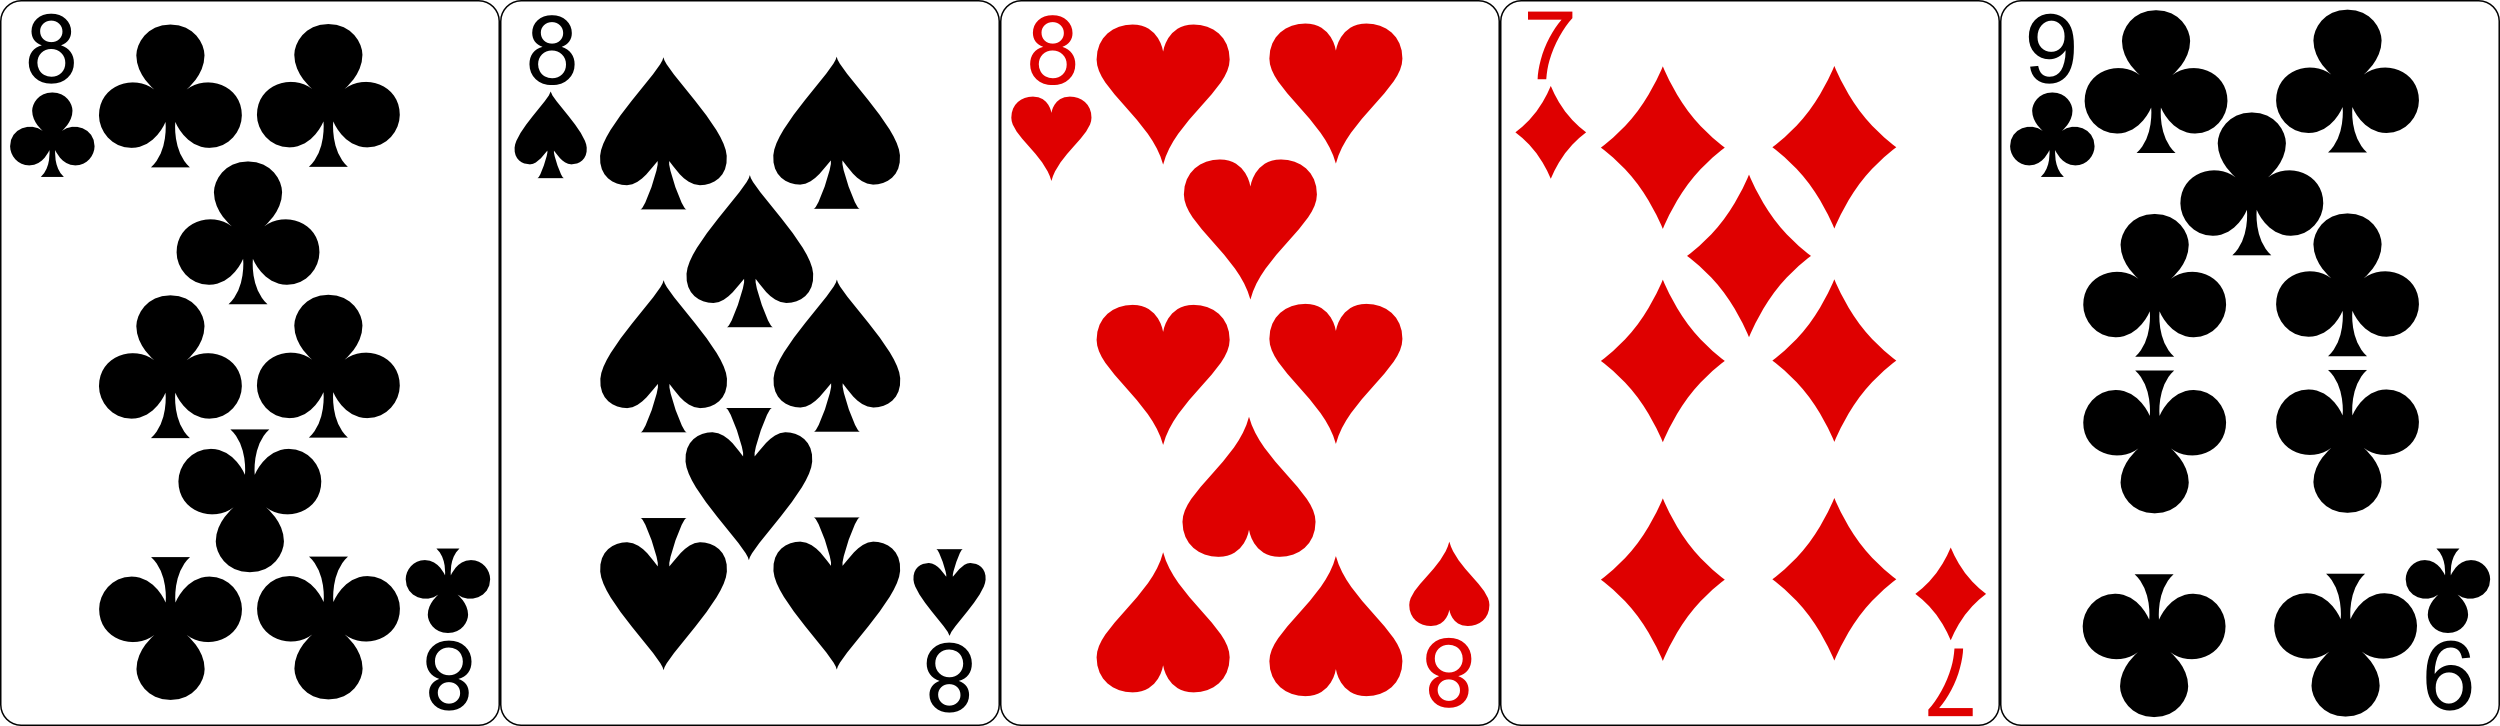
\includegraphics[width=\textwidth]{../img/w05-hands/trips.png}
 \end{minipage}
 \begin{minipage}[c]{0.3\textwidth}
  \caption{Triss - tre kort har samma valör}
 \end{minipage}
\end{figure}

\begin{figure}[H]
 \begin{minipage}[c]{0.5\textwidth}
  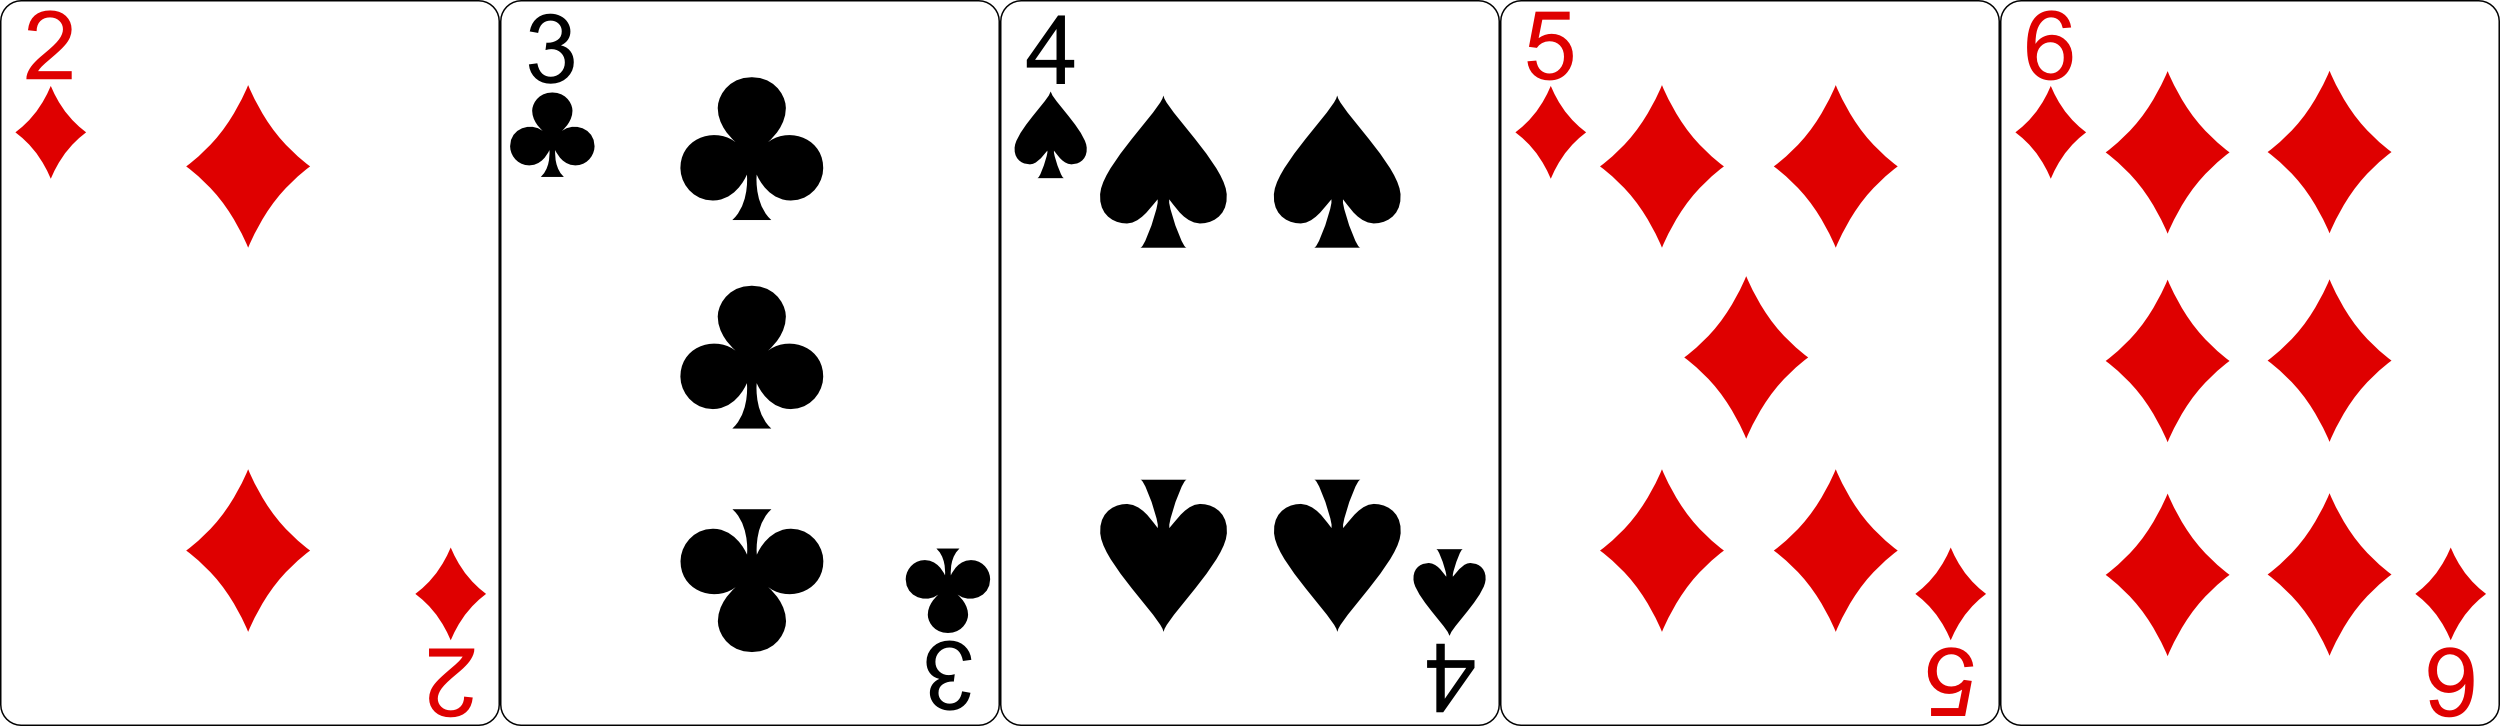
\includegraphics[width=\textwidth]{../img/w05-hands/straight.png}
 \end{minipage}
 \begin{minipage}[c]{0.3\textwidth}
  \caption{Stege - kortens valörer bildar en följd, ess kan vara antingen 1 eller 14}
 \end{minipage}
\end{figure}

\begin{figure}[H]
 \begin{minipage}[c]{0.5\textwidth}
  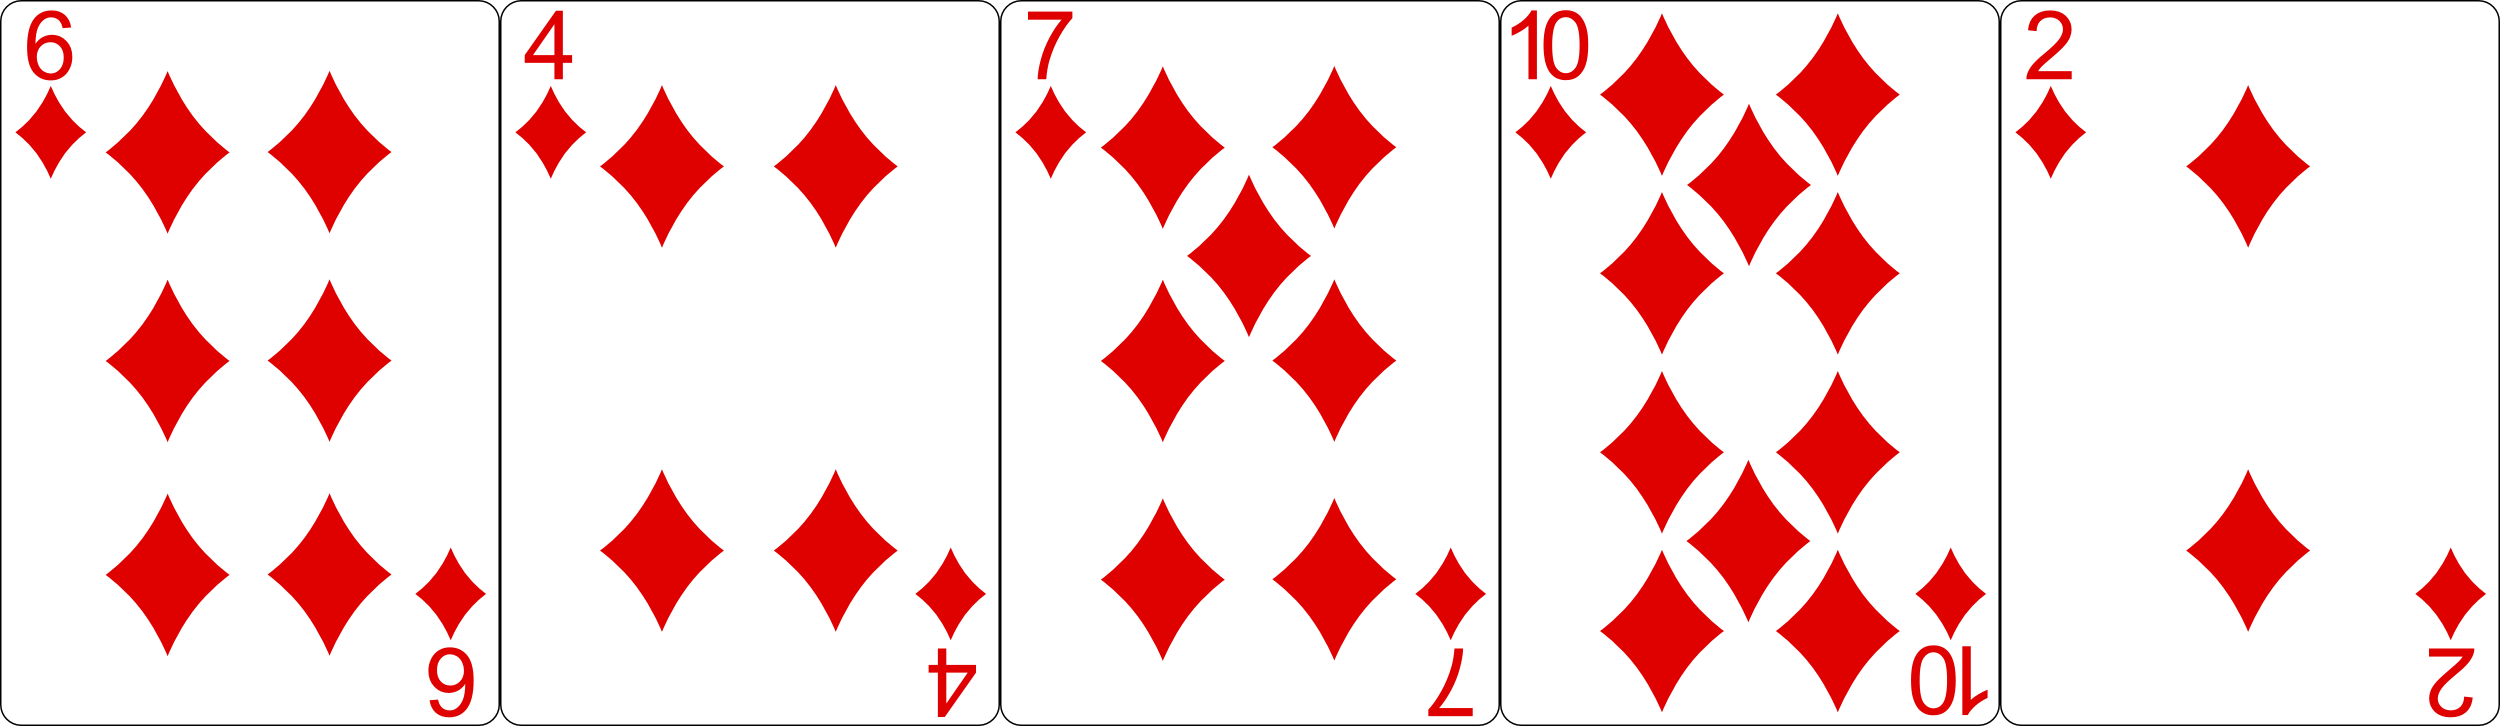
\includegraphics[width=\textwidth]{../img/w05-hands/flush.png}
 \end{minipage}
 \begin{minipage}[c]{0.3\textwidth}
  \caption{Färg - alla kort har samma färg}
 \end{minipage}
\end{figure}

\begin{figure}[H]
 \begin{minipage}[c]{0.5\textwidth}
  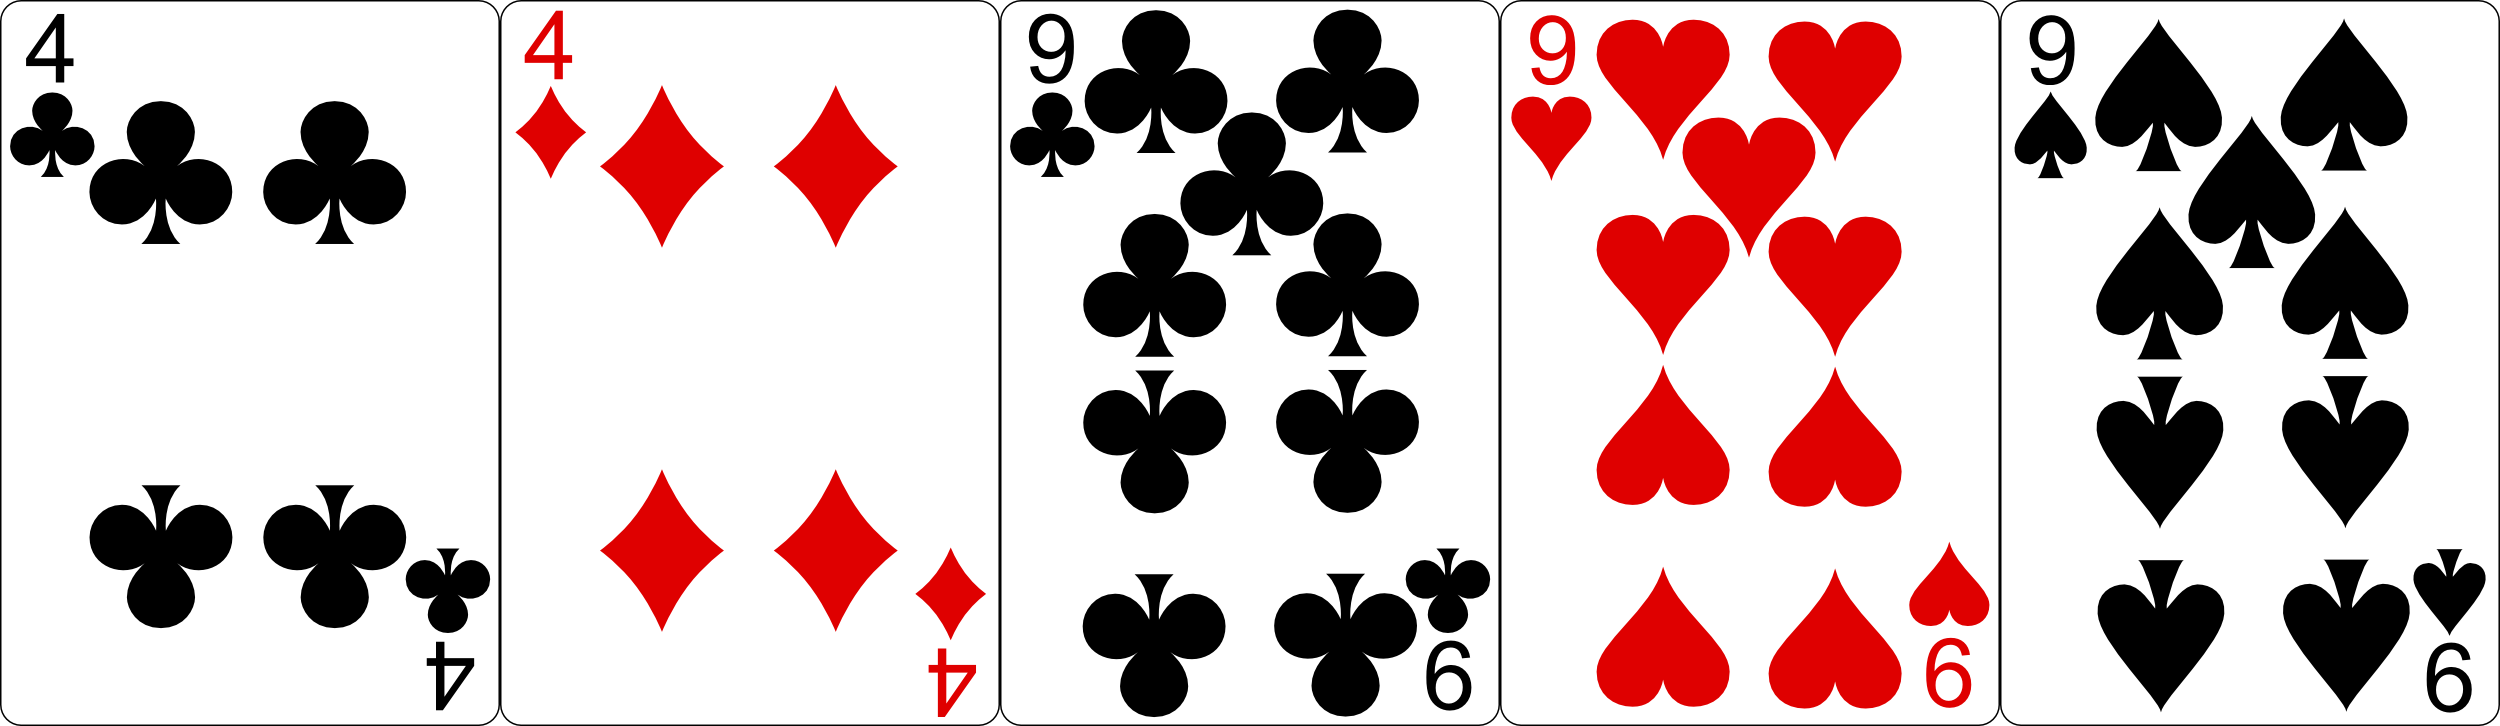
\includegraphics[width=\textwidth]{../img/w05-hands/fullhouse.png}
 \end{minipage}
 \begin{minipage}[c]{0.3\textwidth}
  \caption{Kåk - både triss och par}
 \end{minipage}
\end{figure}

\begin{figure}[H]
 \begin{minipage}[c]{0.5\textwidth}
  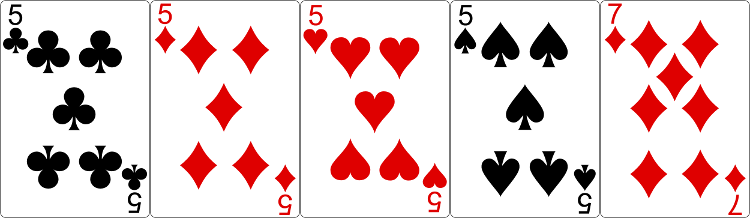
\includegraphics[width=\textwidth]{../img/w05-hands/fours.png}
 \end{minipage}
 \begin{minipage}[c]{0.3\textwidth}
  \caption{Fyrtal - fyra kort har samma valör}
 \end{minipage}
\end{figure}

\begin{figure}[H]
 \begin{minipage}[c]{0.5\textwidth}
  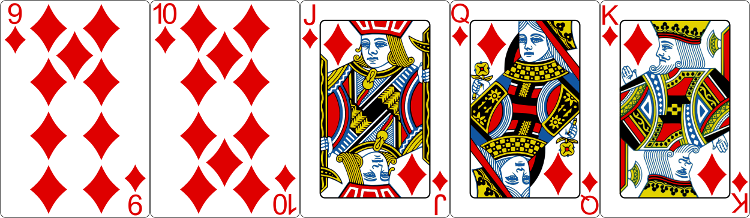
\includegraphics[width=\textwidth]{../img/w05-hands/straightflush.png}
 \end{minipage}
 \begin{minipage}[c]{0.3\textwidth}
  \caption{Färgstege - både stege och färg}
 \end{minipage}
\end{figure}

\begin{figure}[H]
 \begin{minipage}[c]{0.5\textwidth}
  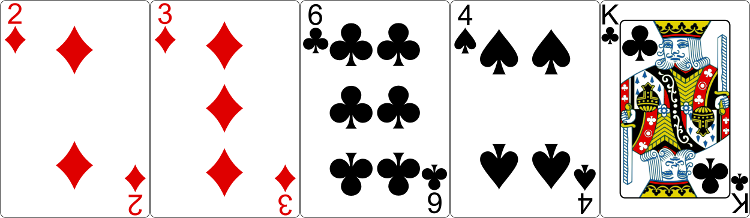
\includegraphics[width=\textwidth]{../img/w05-hands/none.png}
 \end{minipage}
 \begin{minipage}[c]{0.3\textwidth}
  \caption{Högt kort - inget mönster finns}
 \label{lab:shuffle:last-picture}
  \end{minipage}
\end{figure}


